\documentclass[12pt]{article}
%\usepackage{ucs}
\usepackage{amsmath,amssymb,amsthm}
%\usepackage{pb-diagram}
\usepackage{multicol}
\usepackage{color}
\usepackage{graphicx}
\usepackage{epstopdf}
\usepackage{hyperref}

%\usepackage{verbatim}
%\newenvironment{comment}
%{\par\noindent{\bf TODO}\\}
%{\\\hfill$\scriptstyle\blacksquare$\par}

\newtheorem{statement}{Statement}
\newtheorem{theorem}{Theorem}
\newtheorem{corollary}{Corollary}[theorem]
\newtheorem{lemma}{Lemma}
\newtheorem{mynote}{Note}[section]
\theoremstyle{definition}
\newtheorem{definition}{Definition}
\newtheorem{remark}{Remark}
\newcommand{\go}{\stackrel{\circ }{\mathfrak{g}}}
\newcommand{\ao}{\stackrel{\circ }{\mathfrak{a}}}
\newcommand{\co}[1]{\stackrel{\circ }{#1}}
\newcommand{\pia}{\pi_{\mathfrak{a}}}
\newcommand{\piab}{\pi_{\mathfrak{a}_{\bot}}}

\newcommand{\gf}{\mathfrak{g}}
\newcommand{\af}{\mathfrak{a}}
\newcommand{\afb}{\mathfrak{a}_{\bot}}
\newcommand{\hf}{\mathfrak{h}}
\newcommand{\hfb}{\mathfrak{h}_{\bot}}
\newcommand{\pf}{\mathfrak{p}}

\begin{document}
\title{Nope}
\author{V D Lyakhovsky$^1$ and A A Nazarov$^2$}

\begin{abstract}
\end{abstract}

\section{Introduction}

\label{sec:introduction}

The branching properties of Lie (affine Lie) algebras are highly important for
applications in quantum field theory. This concernes for example the
conformal field theory models \cite{difrancesco1997cft},\cite
{coquereaux2008conformal}.

% There are different approaches to deal with the branching coefficients. Some
% of them use the BGG resolution \cite{bernstein1975differential} (for
% Kac-Moody algebras the algorithm is described in \cite{kac1990idl},\cite
% {wakimoto2001idl}).

In this paper we demonstrate that for an arbitrary reductive subalgebra
branching is directly connected with the BGG resolution and in particular
exhibits the resolution properties in terms of the $\mathcal{O}^{p}$
category \cite{lepowsky1977generalization} (the parabolic generalization of the cathegory $%
\mathcal{O}$ \cite{bernstein1976category}).

To show this we use the recursive approach to branching presented in \cite{2010arXiv1007.0318L} (similar to the one used in \cite{ilyin812pbc} for maximal
embeddings). We consider the subalgebra $\frak{a}$ together with its
counterpart $\frak{a}_{\bot }$ ''orthogonal'' to $\frak{a}$ with respect to
the Killing form and also $\widetilde{\frak{a}_{\perp }}:=\frak{a}_{\perp
}\oplus \frak{h}_{\perp }$ where $\frak{h}=\frak{\frak{h}_{\frak{a}}}\oplus 
\frak{h}_{\frak{a}_{\perp }}\oplus \frak{h}_{\perp }$. For any reductive
algebra $\frak{a}$ the subalgebra $\frak{a}_{\bot }\hookrightarrow \frak{g}$
is regular and reductive. For a highest weight integrable module $L^{\left(
\mu \right) }$ and orthogonal pair of subalgebras $\left( \frak{a},\frak{a}%
_{\bot }\right) $ we consider the singular element $\Psi ^{\left( \mu
\right) }$ (the numerator in the Weyl character formula $ch\left( L^{\mu
}\right) =\frac{\Psi ^{\left( \mu \right) }}{\Psi ^{\left( 0\right) }}$, see
for example \cite{humphreys1997introduction}) the Weyl denominator $\Psi _{%
\frak{a}_{\bot }}^{\left( 0\right) }$ and the projection $\Psi _{\left(
\frak{a},\frak{a}_{\bot }\right) }^{\left( \mu \right) }=\pi _{\frak{a}}%
\frac{\Psi _{\frak{g}}^{\left( \mu \right) }}{\Psi _{\frak{a}_{\bot
}}^{\left( 0\right) }}$. The element $\Psi _{\frak{g}}^{\left( \mu \right) }$
can be decomposed with respect to the set of Weyl numerators $\Psi _{\frak{a}%
_{\bot }}^{\left( \mu \right) }$ of $\frak{a}_{\bot }$. This decomposition
provides the possibility to construct the set of highest weight modules $L_{%
\widetilde{\frak{a}_{\perp }}}^{\mu _{\widetilde{\frak{a}_{\perp }}}}$. When
the injection \ $\frak{a}_{\bot }\hookrightarrow \frak{g}$ \ satisfies the
''standard parabolic'' conditions these modules give rise to the parabolic
Verma modules $M_{\left( \widetilde{\frak{a}_{\perp }}\hookrightarrow \frak{g%
}\right) }^{\mu _{\widetilde{\frak{a}_{\perp }}}}$ so that the initial
character $ch\left( L^{\mu }\right) $ is finally decomposed into the
alternating sum of such. On the other hand when the parabolic conditions are
violated the construction survives and exhibites a decomposition with
respect to a set of Verma modules $M_{\left( \widetilde{\frak{b}_{\perp }},%
\frak{g}\right) }^{\mu _{\widetilde{\frak{a}_{\perp }}}}$. In such a
situation the algebra $\widetilde{\frak{b}_{\perp }}$ is not a subalgebra in 
$\frak{g}$ but a contraction of $\widetilde{\frak{a}_{\perp }}$.

Some general properties of the proposed decompositions are formulated in
terms of a specific element $\Gamma _{\frak{a}\rightarrow \frak{g}}$ of the
group algebra $\mathcal{E}\left( \frak{g}\right) $ called ''the injection
fan''. Using this tool the simple and explicit algorithm for branching
coefficients computations applicable for an arbitrary (maximal or
nonmaximal) subalgebras of finite-dimensional or affine Lie algebras was
obtained in \cite{2010arXiv1007.0318L}.

Possible further developments are discussed in Section \ref{sec:conclusion}.

\subsection{Notation}

\label{sec:notation}

Consider affine Lie algebras $\frak{g}$ and $\frak{a}$ with the underlying
finite-dimensional subalgebras $\stackrel{\circ }{\frak{g}}$ and $\stackrel{%
\circ }{\frak{a}}$ and an injection $\frak{a}\hookrightarrow \frak{g}$ such
that $\frak{a}$ is a reductive subalgebra $\frak{a\subset g}$ with
correlated root spaces: $\frak{h}_{\frak{a}}^{\ast }\subset \frak{h}_{\frak{g%
}}^{\ast }$ and $\frak{h}_{\stackrel{\circ }{\frak{a}}}^{\ast }\subset \frak{%
h}_{\stackrel{\circ }{\frak{g}}}^{\ast }$\ . We use the following notations:

$\frak{g=n}^{-}+\frak{b}+\frak{n}^{+}$ --- the Cartan decomposition;

$r$ , $\left( r_{\frak{a}}\right) $ --- the rank of the algebra $\frak{g}$ $%
\left( \mathrm{{resp. }\frak{a}}\right) $ ;

$\Delta $ $\left( \Delta _{\frak{a}}\right) $--- the root system; $\Delta
^{+} $ $\left( \mathrm{{resp. }\Delta _{\frak{a}}^{+}}\right) $--- the
positive root system (of $\frak{g}$ and $\frak{a}$ respectively);

$\mathrm{mult}\left( \alpha \right) $ $\left( \mathrm{mult}_{\frak{a}}\left(
\alpha \right) \right) $ --- the multiplicity of the root $\alpha$ in $%
\Delta $ (resp. in $\left( \Delta _{\frak{a}}\right) $);

$S\quad \left( S_{\frak{a}}\right) $ --- the system of simple roots (of $%
\frak{g}$ and $\frak{a}$ respectively);

$\stackrel{\circ }{\Delta }$ , $\left( \stackrel{\circ }{\Delta _{\frak{a}}}%
\right) $ --- the finite root system of the subalgebra $\stackrel{\circ }{%
\frak{g}}$ (resp. $\stackrel{\circ }{\frak{a}}$);

$\alpha _{i}$ , $\left( \alpha _{\left( \frak{a}\right) j}\right) $ --- the $%
i$-th (resp. $j$-th) basic root for $\frak{g}$ $\left( \mathrm{{resp.}\frak{a%
}}\right) $; $i=0,\ldots ,r$,\ \ $\left( j=0,\ldots ,r_{\frak{a}}\right) $;

$\delta $ --- the imaginary root of $\frak{g}$ (and of $\frak{a}$ if any);

$\alpha _{i}^{\vee }$ , $\left( \alpha _{\left( \frak{a}\right) j}^{\vee
}\right) $--- the basic coroot for $\frak{g}$ $\left( \mathrm{{resp.}\frak{a}%
}\right) $ , $i=0,\ldots ,r$ ;\ \ $\left( j=0,\ldots ,r_{\frak{a}}\right) $;

$W$ , $\left( W_{\frak{a}}\right) $--- the corresponding Weyl group;

$C$ , $\left( C_{\frak{a}}\right) $--- the fundamental Weyl chamber;

$\bar{C}, \left(\bar{C_{\frak{a}}}\right)$ --- the closure of the
fundamental Weyl chamber;

$\epsilon \left( w\right) :=\left( -1\right) ^{\mathrm{length}(w)}$;

$\rho $\ , $\left( \rho _{\frak{a}}\right) $\ --- the Weyl vector;

$L^{\mu }$\ $\left( L_{\frak{a}}^{\nu }\right) $\ --- the integrable module
of $\frak{g}$ with the highest weight $\mu $\ ; (resp. integrable $\frak{a}$
-module with the highest weight $\nu $ );

$\mathcal{N}^{\mu }$ , $\left( \mathcal{N}_{\frak{a}}^{\nu }\right) $ ---
the weight diagram of $L^{\mu }$ $\left( \mathrm{{resp.}L_{\frak{a}}^{\nu }}%
\right) $ ;

$\stackrel{\circ }{\xi }$ , $\stackrel{\circ }{\xi _{\left( \frak{a}\right) }%
}$ --- the finite (classical) part of the weight $\xi \in P$ , $\left(
\mathrm{{resp.}\xi _{\left( \frak{a}\right) }\in P_{\frak{a}}}\right) $;

$\lambda =\left( \stackrel{\circ }{\lambda };k;n\right) $ --- the
decomposition of an affine weight indicating the finite part $\stackrel{%
\circ }{\lambda }$, level $k$ and grade $n$;

$P$ $\left( \mathrm{{resp.}P_{\frak{a}}}\right) $ \ --- the weight lattice;

$P^{+}$ $\left( \mathrm{{resp.}P_{\frak{a}}^{+}}\right) $ \ --- the dominant
weight lattice;

$m_{\xi }^{\left( \mu \right) }$ , $\left( m_{\xi }^{\left( \nu \right)
}\right) $ --- the multiplicity of the weight $\xi \in P$ \ $\left( \mathrm{{%
resp. }\in P_{\frak{a}}}\right) $ in the module $L^{\mu }$ , (resp. $\xi \in
L_{\frak{a}}^{\nu } $);

$ch\left( L^{\mu }\right) $ $\left( \mathrm{{resp. }ch\left( L_{\frak{a}%
}^{\nu }\right) }\right) $--- the formal character of $L^{\mu }$ $\left( 
\mathrm{{resp. }L_{\frak{a}}^{\nu }}\right) $;

$ch\left( L^{\mu }\right) =\frac{\sum_{w\in W}\epsilon (w)e^{w\circ (\mu
+\rho )-\rho }}{\prod_{\alpha \in \Delta ^{+}}\left( 1-e^{-\alpha }\right) ^{%
\mathrm{{mult}\left( \alpha \right) }}}$ --- the Weyl-Kac formula;

$R:=\prod_{\alpha \in \Delta ^{+}}\left( 1-e^{-\alpha }\right) ^{\mathrm{{%
mult}\left( \alpha \right) }}\quad $ $\left( \mathrm{resp.}R_{\frak{a}%
}:=\prod_{\alpha \in \Delta _{\frak{a}}^{+}}\left( 1-e^{-\alpha }\right) ^{%
\mathrm{mult}_{\frak{a}}\mathrm{\left( \alpha \right) }}\right) $--- the
Weyl denominator.

\section{Orthogonal subalgebra and the singular element}

\label{sec:recurr-form-branch}

Consider the highest weight $\mu \in P^{+}$ of an integrable module $L^{\mu
} $ of $\frak{g}$ and let $\frak{a}\subset \frak{g}$ be a reductive
subalgebra of $\frak{g}$. Let $L^{\mu }$ be completely reducible with
respect to $\frak{a}$, 
\[
L_{\frak{g}\downarrow \frak{a}}^{\mu }=\bigoplus\limits_{\nu \in P_{\frak{a}%
}^{+}}b_{\nu }^{\left( \mu \right) }L_{\frak{a}}^{\nu }. 
\]
Using the projection operator $\pi _{\frak{a}}$ (to the weight space $\frak{%
h_{a}}^{\ast }$) one can rewrite this decomposition in terms of formal
characters: 
\begin{equation}
\pi _{\frak{a}}ch\left( L^{\mu }\right) =\sum_{\nu \in P_{\frak{a}%
}^{+}}b_{\nu }^{(\mu )}ch\left( L_{\frak{a}}^{\nu }\right) .
\label{branching1}
\end{equation}
The module $L^{\mu }$ has the BGG-resolution (see
\cite{bernstein1976category,bernstein1975differential,bernstein1971structure} and \cite{humphreys2008representations}). All
the members of the filtration sequence are the direct sums of Verma modules
and all their highest weights $\nu $ are strongly linked to $\mu $: 
\[
\left\{ \nu \right\} =\left\{ w\left( \mu +\rho \right) -\rho |w\in
W\right\} . 
\]

\subsection{Orthogonal subalgebra}

Now we shall show how the branching procedure naturally produces the
generalized Verma modules.

Consider in $\frak{g}$ a reductive subalgebra $\frak{a}$ with the Cartan
subalgebra $\frak{h}_{\frak{a}}$. For $\frak{a}\hookrightarrow \frak{g}$
introduce the ''orthogonal partner'' $\frak{a}_{\bot }\hookrightarrow \frak{g%
}$ .

Firstly consider the root subspace $\frak{h}_{\perp \frak{a}}^{\ast }$
orthogonal to $\frak{a}$,
\[
\frak{h}_{\perp \frak{a}}^{\ast }:=\left\{ \eta \in \frak{h}^{\ast }|\forall
h\in \frak{h}_{\frak{a}};\eta \left( h\right) =0\right\} , 
\]
and the roots (correspondingly -- positive roots) of $\frak{g}$ orthogonal
to $\frak{a}$, 
\begin{eqnarray*}
\Delta _{\frak{a}_{\perp }} &:&=\left\{ \beta \in \Delta _{\frak{g}}|\forall
h\in \frak{h}_{\frak{a}};\beta \left( h\right) =0\right\} , \\
\Delta _{\frak{a}_{\perp }}^{+} &:&=\left\{ \beta ^{+}\in \Delta _{\frak{g}%
}^{+}|\forall h\in \frak{h}_{\frak{a}};\beta ^{+}\left( h\right) =0\right\} .
\end{eqnarray*}
Let $W_{\frak{a}_{\perp }}$ be the subgroup of $W$ generated by the
reflections $w_{\beta }$ with the roots $\beta \in \Delta _{\frak{a}_{\perp
}}^{+}$ . The subsystem $\Delta _{\frak{a}_{\perp }}$ determines the
subalgebra $\frak{a}_{\perp }$ with the Cartan subalgebra $\frak{h}_{\frak{a}%
_{\perp }}$. Let 
\[
\frak{h}_{\perp }^{\ast }:=\left\{ \eta \in \frak{h}_{\perp \frak{a}}^{\ast
}|\forall h\in \frak{h}_{\frak{a}\oplus \frak{a}_{\perp }};\eta \left(
h\right) =0\right\} 
\]
so that $\frak{g}$ has the subalgebras 
\begin{eqnarray*}
\widetilde{\frak{a}_{\perp }} &:&=\frak{a}_{\perp }\oplus \frak{h}_{\perp }
\\
\widetilde{\frak{a}} &:&=\frak{a}\oplus \frak{h}_{\perp }.
\end{eqnarray*}

For the Cartan subalgebras we have the decomposition 
\begin{equation}
\frak{h}=\frak{\frak{h}_{\frak{a}}}\oplus \frak{h}_{\frak{a}_{\perp }}\oplus 
\frak{h}_{\perp }=\frak{\frak{h}_{\widetilde{\frak{a}}}}\oplus \frak{h}_{%
\frak{a}_{\perp }}=\frak{\frak{h}_{\widetilde{\frak{a}_{\perp }}}}\oplus 
\frak{h}_{\frak{a}}.
\end{equation}
For the subalgebras $\frak{a}$ and $\frak{a}_{\perp }$ consider the
corresponding Weyl vectors, $\rho _{\frak{a}}$ and $\rho _{\frak{a}_{\perp }}
$ , and\ form the so called ''defects'' $\mathcal{D}_{\frak{a}}$ and $%
\mathcal{D}_{\frak{a}_{\perp }}$ of the injection:
\begin{equation}
\mathcal{D}_{\frak{a}}:=\rho _{\frak{a}}-\pi _{\frak{a}}\rho ,
\end{equation}
\begin{equation}
\mathcal{D}_{\frak{a}_{\perp }}:=\rho _{\frak{a}_{\perp }}-\pi _{\frak{a}%
_{\perp }}\rho .  \label{defect ort}
\end{equation}

For the highest weight $\mu \in P^{+}$ consider the linked weights $\left\{
\left( w(\mu +\rho )-\rho \right) |w\in W\right\} $ and their projections to 
$h_{\widetilde{\frak{a}_{\perp }}}^{\ast }$ additionally shifted by the
defect $-\mathcal{D}_{\frak{a}_{\perp }}$: 
\[
\mu _{\widetilde{\frak{a}_{\perp }}}\left( w\right) :=\pi _{\widetilde{\frak{%
a}_{\perp }}}\left[ w(\mu +\rho )-\rho \right] -\mathcal{D}_{\frak{a}_{\perp
}},\quad w\in W. 
\]
For $\mu \in P^{+}$ among the weights $\left\{ \mu _{\widetilde{\frak{a}%
_{\perp }}}\left( w\right) |w\in W\right\} $ one can always choose those
located in the fundamental chamber $\overline{C_{\widetilde{\frak{a}_{\perp }%
}}}$. Let $U$ be the set of representatives $u$ for the classes $W/W_{\frak{a%
}_{\perp }}$ such that

\begin{equation}
U:=\left\{ u\in W|\quad \mu _{\widetilde{\frak{a}_{\perp }}}\left( u\right)
\in \overline{C_{\widetilde{\frak{a}_{\perp }}}}\right\} \quad .
\label{U-def}
\end{equation}
Thus we can select the following subsets:
\begin{equation}
\mu _{\frak{a}}\left( u\right) :=\pi _{\frak{a}}\left[ u(\mu +\rho )-\rho %
\right] +\mathcal{D}_{\frak{a}_{\perp }},\quad u\in U,  \label{mu-a}
\end{equation}
and
\begin{equation}
\mu _{\widetilde{\frak{a}_{\perp }}}\left( u\right) :=\pi _{\widetilde{\frak{%
a}_{\perp }}}\left[ u(\mu +\rho )-\rho \right] -\mathcal{D}_{\frak{a}_{\perp
}},\quad u\in U.  \label{mu-a-tilda}
\end{equation}

Note that the subalgebra $\afb$ is regular by definition since it is built on the roots of the
algebra $\gf$.

For the modules we are interested in the Weyl-Kac formula for $ch\left( L^{\mu }\right) $ can be
written in terms of
singular elements \cite{humphreys1997introduction}
\[
\Psi ^{\left( \mu \right) }:=\sum\limits_{w\in W}\epsilon (w)e^{w\circ (\mu
+\rho )-\rho },
\]
namely,
\begin{equation}
ch\left( L^{\mu }\right) =\frac{\Psi ^{\left( \mu \right) }}{\Psi ^{\left(
0\right) }}=\frac{\Psi ^{\left( \mu \right) }}{R}.  \label{Weyl-Kac2}
\end{equation}
The same is true for the submodules $ch\left( L_{\frak{a}}^{\nu }\right) $
in (\ref{branching1})
\[
ch\left( L_{\frak{a}}^{\nu }\right) =\frac{\Psi _{\frak{a}}^{\left( \nu
\right) }}{\Psi _{\frak{a}}^{\left( 0\right) }}=\frac{\Psi _{\frak{a}%
}^{\left( \nu \right) }}{R_{\frak{a}}}, 
\]
with 
\[
\Psi _{\frak{a}}^{\left( \nu \right) }:=\sum\limits_{w\in W_{\frak{a}%
}}\epsilon (w)e^{w\circ (\nu +\rho _{_{\frak{a}}})-\rho _{_{\frak{a}}}}. 
\]

Applying formula (\ref{Weyl-Kac2}) to the branching rule (\ref{branching1})
we get the relation connecting the singular elements $\Psi ^{\left( \mu
\right) }$ and $\Psi _{\frak{a}}^{\left( \nu \right) }$ : 
\begin{eqnarray}
\pi _{\frak{a}}\left( \frac{\sum_{w \in W}\epsilon (w )e^{w (\mu +\rho
)-\rho }}{\prod_{\alpha \in \Delta ^{+}}(1-e^{-\alpha })^{\mathrm{mult}%
(\alpha )}}\right) &=&\sum_{\nu \in P_{\frak{a}}^{+}}b_{\nu }^{(\mu )}\frac{%
\sum_{w \in W_{\frak{a}}}\epsilon (w )e^{w (\nu +\rho _{\frak{a}})-\rho _{%
\frak{a}}}}{\prod_{\beta \in \Delta _{\frak{a}}^{+}}(1-e^{-\beta })^{\mathrm{%
mult}_{\frak{a}}(\beta )}},  \nonumber  \label{eq:4} \\
\pi _{\frak{a}}\left( \frac{\Psi ^{\left( \mu \right) }}{R}\right)
&=&\sum_{\nu \in P_{\frak{a}}^{+}}b_{\nu }^{(\mu )}\frac{\Psi _{\frak{a}%
}^{\left( \nu \right) }}{R_{\frak{a}}}.
\end{eqnarray}
Here $\Delta _{\frak{a}}^{+}$ is the set of positive roots of the subalgebra 
$\frak{a}$ (without loss of generality we consider them as vectors from the
positive root space $\frak{h}^{\ast +}$ of $\frak{g}$).

\subsection{Decomposing the singular element.}

\label{subsec:decomp-sing-element}

Now we shall perform a decomposition of the singular element $\Psi ^{\left(
\mu \right) }$ in terms of singular elements of the orthogonal subalgebra
modules:

\begin{lemma}
Let $\frak{a}_{\bot }$ be the orthogonal partner of a reductive subalgebra $%
\frak{a}\hookrightarrow \frak{g}$ with $\frak{h}=\frak{\frak{h}_{\frak{a}}}%
\oplus \frak{h}_{\frak{a}_{\perp }}\oplus \frak{h}_{\perp }$, $\widetilde{%
\frak{a}_{\perp }}=\frak{a}_{\perp }\oplus \frak{h}_{\perp }$ and $%
\widetilde{\frak{a}}=\frak{a}\oplus \frak{h}_{\perp }$.

$L^{\mu }$ be the highest weight integrable module with $\mu \in P^{+}$ and

$\Psi ^{\left( \mu \right) }$\ -- the singular element of $L^{\mu }$.

Then the element $\Psi ^{\left( \mu \right) }$ can be decomposed into the
sum over $u\in U$ (see (\ref{U-def})) of singular elements $\Psi _{%
\widetilde{\frak{a}_{\perp }}}^{\mu _{\widetilde{\frak{a}_{\perp }}}\left(
u\right) }$ with the coefficients $\epsilon (u)e^{\mu _{\frak{a}}\left(
u\right) }$:
\begin{equation}
\Psi ^{\left( \mu \right) }=\sum_{u\in U}\;\epsilon (u)e^{\mu _{\frak{a}%
}\left( u\right) }\Psi _{\widetilde{\frak{a}_{\perp }}}^{\mu _{\widetilde{%
\frak{a}_{\perp }}}\left( u\right) }.  \label{sing decomp main}
\end{equation}
\end{lemma}

\begin{proof}
With $u\in U$ and $v\in W_{\frak{a}_{\bot }}$ perform the decomposition
\[
u(\mu +\rho )=\pi _{\left( \frak{a}\right) }u(\mu +\rho )+\pi _{\left(
\widetilde{\frak{a}_{\perp }}\right) }u(\mu +\rho )
\]
for the singular weight $vu(\mu +\rho )-\rho $:
\begin{equation}
\begin{array}{lcl}
vu(\mu +\rho )-\rho  & = & \pi _{\left( \frak{a}\right) }\left( u(\mu +\rho
)\right) -\rho +\rho _{\frak{a}_{\perp }}+\pi _{\left( \frak{h}_{\bot
}\right) }\rho  \\
&  & +\ v\left( \pi _{\left( \widetilde{\frak{a}_{\perp }}\right) }u(\mu
+\rho )-\rho _{\frak{a}_{\perp }}+\rho _{\frak{a}_{\perp }}\right) -\rho _{%
\frak{a}_{\perp }}-\pi _{\left( \frak{h}_{\bot }\right) }\rho .
\end{array}
\label{sing-decomp-1}
\end{equation}
Use the defect $\mathcal{D}_{\frak{a}_{\bot }}$ (\ref{defect-perp}) to
simplify the first summand in (\ref{sing-decomp-1}):
\[
\begin{array}{r}
\pi _{\left( \frak{a}\right) }\left( u(\mu +\rho )\right) -\rho +\rho _{%
\frak{a}_{\perp }}+\pi _{\left( \frak{h}_{\bot }\right) }\rho = \\
\pi _{\left( \frak{a}\right) }\left( u(\mu +\rho )\right) -\pi _{\frak{a}%
}\rho -\pi _{\frak{a}_{\bot }}\rho +\rho _{\frak{a}_{\bot }}= \\
=\pi _{\left( \frak{a}\right) }\left( u(\mu +\rho )-\rho \right) +\mathcal{D}%
_{\frak{a}_{\bot }},
\end{array}
\]
and the second one:
\[
\begin{array}{c}
v\left( \pi _{\left( \widetilde{\frak{a}_{\perp }}\right) }u(\mu +\rho
)-\rho _{\frak{a}_{\perp }}+\rho _{\frak{a}_{\perp }}\right) -\rho _{\frak{a}%
_{\perp }}-\pi _{\left( \frak{h}_{\bot }\right) }\rho = \\
v\left( \pi _{\left( \widetilde{\frak{a}_{\bot }}\right) }u(\mu +\rho )-%
\mathcal{D}_{\frak{a}_{\bot }}-\pi _{\left( \frak{a}_{\bot }\right) }\rho
-\pi _{\left( \frak{h}_{\bot }\right) }\rho +\rho _{\frak{a}_{\bot }}\right)
-\rho _{\frak{a}_{\bot }}= \\
=v\left( \pi _{\left( \widetilde{\frak{a}_{\bot }}\right) }\left[ u(\mu
+\rho )-\rho \right] -\mathcal{D}_{\frak{a}_{\bot }}+\rho _{\frak{a}_{\bot
}}\right) -\rho _{\frak{a}_{\bot }}.
\end{array}
\]
These expressions provide the desired factorization of the singular element $%
\Psi ^{\mu }$ in terms of singular elements $\Psi _{\widetilde{\frak{a}%
_{\perp }}}^{\eta }$ of the $\widetilde{\frak{a}_{\perp }}$-modules $L_{%
\widetilde{\frak{a}_{\perp }}}^{\eta }$:
\begin{equation}
\begin{array}{l}
\Psi ^{\mu }=\sum_{u\in U}\sum_{v\in W_{\frak{a}_{\perp }}}\epsilon
(v)\epsilon (u)e^{vu(\mu +\rho )-\rho }= \\
=\sum_{u\in U}\epsilon (u)e^{\pi _{\frak{a}}\left[ u(\mu +\rho )-\rho \right]
+\mathcal{D}_{\frak{a}_{\perp }}}\sum_{v\in W_{\frak{a}_{\perp }}}\epsilon
(v)e^{v\left( \pi _{\left( \widetilde{\frak{a}_{\perp }}\right) }\left[
u(\mu +\rho )-\rho \right] -\mathcal{D}_{\frak{a}_{\perp }}+\rho _{\frak{a}%
_{\perp }}\right) -\rho _{\frak{a}_{\perp }}}= \\
=\sum_{u\in U}\;\epsilon (u)\Psi _{\widetilde{\frak{a}_{\perp }}}^{\pi
_{\left( \widetilde{\frak{a}_{\perp }}\right) }\left[ u(\mu +\rho )-\rho
\right] -\mathcal{D}_{\frak{a}_{\perp }}}e^{\pi _{\left( \frak{a}\right) }%
\left[ u(\mu +\rho )-\rho \right] +\mathcal{D}_{\frak{a}_{\perp }}}.
\end{array}
\label{singular main}
\end{equation}
\end{proof}

\bigskip

\begin{remark}
This relation can be considered as a generalized form of the Weyl formula
for the singular element $\Psi _{\frak{g}}^{\mu }$: the vectors $\mu _{\frak{%
a}}\left( u\right) $ play the role of singular weights while the alternating
factors $\epsilon (u)$ are extended to $\epsilon (u)\Psi _{\widetilde{\frak{a%
}_{\perp }}}^{\mu _{\widetilde{\frak{a}_{\perp }}}\left( u\right) }$. In
fact when $\frak{a=g}$ both $\frak{a}_{\perp }$and $\frak{h}_{\perp }$are
zeros, $U=W$, and\ the original Weyl formula is reobtained via the
trivilization of the singular elements: $\epsilon (u)\Psi _{\widetilde{\frak{%
a}_{\perp }}}^{\mu _{\widetilde{\frak{a}_{\perp }}}\left( u\right)
}=\epsilon (u)$. In the opposite limit when $\frak{a=0}$, $\Delta _{\frak{a}%
_{\perp }}=\Delta _{\frak{g}}$, $\frak{h}_{\perp }^{\ast }=0$, $\widetilde{%
\frak{a}_{\perp }}=\frak{g}$, $\mathcal{D}_{\frak{a}_{\perp }}=0$, $U=W/W_{%
\frak{a}_{\perp }}=e$ and $\Psi ^{\mu }$ is again reobtained, now via the
trivilization of the set of vectors: $\mu _{\frak{a}}\left( e\right) =0$.
\end{remark}

\begin{remark}
In [our preprint] the decomposition analogous to (\ref{singular main}) was
used to construct the recurrent relations for branching coefficients $k_{\xi
}^{\left( \mu \right) }$ corresponding to the injection $\frak{a}%
\hookrightarrow \frak{g}$:
\[
\begin{array}{c}
k_{\xi }^{\left( \mu \right) }=-\frac{1}{s\left( \gamma _{0}\right) }\left(
\sum_{u\in U}\epsilon (u)\;\dim \left( L_{\widetilde{\frak{a}_{\perp }}%
}^{\mu _{\widetilde{\frak{a}_{\perp }}}\left( u\right) }\right) \delta _{\xi
-\gamma _{0},\pi _{\frak{a}}(u(\mu +\rho )-\rho )}+\right.  \\
\left. +\sum_{\gamma \in \Gamma _{\frak{a}\rightarrow \frak{g}}}s\left(
\gamma +\gamma _{0}\right) k_{\xi +\gamma }^{\left( \mu \right) }\right) .
\end{array}
\]
The recursion is goverened by the set $\Gamma _{\frak{a}\rightarrow \frak{g}}
$ called the injection fan. The latter is defined the carrier set $\left\{
\xi \right\} _{\frak{a}\rightarrow \frak{g}}$ for the coefficient function $%
s(\xi )$
\[
\left\{ \xi \right\} _{\frak{a}\rightarrow \frak{g}}:=\left\{ \xi \in P_{%
\frak{a}}|s(\xi )\neq 0\right\}
\]
appearing in the expansion
\begin{equation}
\prod_{\alpha \in \Delta ^{+}\setminus \Delta _{\bot }^{+}}\left( 1-e^{-\pi
_{\frak{a}}\alpha }\right) ^{\mathrm{mult}(\alpha )-\mathrm{mult}_{\frak{a}%
}(\pi _{\frak{a}}\alpha )}=-\sum_{\gamma \in P_{\frak{a}}}s(\gamma
)e^{-\gamma };\quad
\end{equation}
The weights in $\left\{ \xi \right\} _{\frak{a}\rightarrow \frak{g}}$ are to
be shifted by $\gamma _{0}$ -- the lowest vector in $\left\{ \xi \right\} $
-- and the zero element is to be eliminated:
\begin{equation}
\Gamma _{\frak{a}\rightarrow \frak{g}}=\left\{ \xi -\gamma _{0}|\xi \in
\left\{ \xi \right\} \right\} \setminus \left\{ 0\right\} .
\end{equation}
\end{remark}

\subsection{Weyl like formulas.}

\bigskip By the definition the subalgebra $\widetilde{\frak{a}_{\perp }}$ is
regular and reductive. Consider its Weyl denominator $R_{\widetilde{\frak{a}%
_{\perp }}}:=\prod_{\alpha \in \Delta _{\widetilde{\frak{a}_{\perp }}%
}^{+}}\left( 1-e^{-\alpha }\right) ^{\mathrm{mult}_{\frak{a}}\mathrm{\left(
\alpha \right) }}$ and the element $R_{J}:=\prod_{\alpha \in \Delta
^{+}\setminus \Delta _{\widetilde{\frak{a}_{\perp }}}^{+}}\left(
1-e^{-\alpha }\right) ^{\mathrm{mult}(\alpha )}$ as the factors in $R$: $%
\quad $%
\[
R=R_{J}R_{\widetilde{\frak{a}_{\perp }}}.
\]
According to this factorization and the decomposition (\ref{sing decomp main}%
) the character $ch\left( L^{\mu }\right) $ can be written as
\begin{eqnarray*}
\mathrm{ch}\left( L^{\mu }\right) &=&\left( R_{J}\right) ^{-1}\left( R_{%
\widetilde{\frak{a}_{\perp }}}\right) ^{-1}\Psi ^{\mu }=\left( R_{J}\right)
^{-1}\sum_{u\in U}\;e^{\mu _{\frak{a}}\left( u\right) }\epsilon (u)\left( R_{%
\widetilde{\frak{a}_{\perp }}}\right) ^{-1}\Psi _{\widetilde{\frak{a}_{\perp
}}}^{\mu _{\widetilde{\frak{a}_{\perp }}}\left( u\right) } \\
&=&\left( R_{J}\right) ^{-1}\sum_{u\in U}\;e^{\mu _{\frak{a}}\left( u\right)
}\epsilon (u)L_{\widetilde{\frak{a}_{\perp }}}^{\mu _{\widetilde{\frak{a}%
_{\perp }}}\left( u\right) },
\end{eqnarray*}
where $\left\{ L_{\widetilde{\frak{a}_{\perp }}}^{\mu _{\widetilde{\frak{a}%
_{\perp }}}\left( u\right) }|u\in U\right\} $ is the set of
finite-dimensional $\widetilde{\frak{a}_{\perp }}$-modules with the highest
weights $\mu _{\widetilde{\frak{a}_{\perp }}}\left( u\right) $.

Now remember that the subalgebra $\widetilde{\frak{a}_{\perp }}$ is regular
and reductive. We are interested in nontrivial subalgebras $\frak{a}$ and
correspondingly in nontrivial $\widetilde{\frak{a}_{\perp }}$ (the case of a
trivial orthogonal subalgebra arise when $\frak{a}=\frak{g}$ and was
considered above (see Remark 1)). This means that $r_{\frak{a}}\geq 1$ and $%
r_{\widetilde{\frak{a}_{\perp }}}<r$. Due to the fact that any maximal
regular subalgebra has the Dynkin scheme obtained by one or two node
subtractions from the extended Dynkin scheme and the extended scheme has at
most one dependent root (the highest root) the set of roots $\Delta _{%
\widetilde{\frak{a}_{\perp }}}^{+}$ is always equivalent to the one $\Delta
_{I}^{+}$ generated\ by some subset $I\subset S$ of simple roots.

It follows that we can (by redefining the set $\Delta ^{+}$) identify $%
\Delta _{\widetilde{\frak{a}_{\perp }}}^{+}$ with the subset $\Delta _{I}^{+}
$ \ where $I\subset S$ . This allows us to introduce the elements necessary
to compose the generalized Verma modules [Lepowsky,Hamphrys]. We have two
sets of root vectors $\left\{ x_{\xi }\in \frak{g}_{\xi }|\xi \in \Delta
_{I}^{+}\right\} $ and $\left\{ x_{\eta }\in \frak{g}_{\eta }|\eta \in
\Delta ^{+}\setminus \Delta _{I}^{+}\right\} $ . They generate nilpotent
subalgebras of $\frak{n}^{+}$:
\[
\frak{n}_{I}^{+}:=\sum_{\xi \in \Delta _{I}^{+}}\frak{g}_{\xi },\quad \frak{u%
}_{I}^{+}:=\sum_{\eta \in \Delta ^{+}\setminus \Delta _{I}^{+}}\frak{g}%
_{\eta }.
\]
The first subalgebra together with its negative counterpart $\frak{n}_{I}^{-}
$ generates a simple subalgebra
\[
\frak{s}_{I}=\frak{n}_{I}^{-}+\frak{h}_{I}+\frak{n}_{I}^{+}.
\]
We enlarge it with the remaining Cartan generators and introduce the
subalgebra:
\[
\frak{l}_{I}=\frak{n}_{I}^{-}+\frak{h}+\frak{n}_{I}^{+}.
\]
The semidirect product of subalgebras $\frak{l}_{I}$ and $\frak{u}_{I}^{+}$
gives a parabolic subalgebra in $\frak{g}$ :
\begin{equation}
\frak{p}_{I}=\frak{l}_{I}\vartriangleright \frak{u}_{I}^{+},
\label{paralolic subalg}
\end{equation}
Its universal enveloping $U\left( \frak{p}_{I}\right) $ is a subalgebra in $%
U\left( \frak{g}\right) $. According to the obtained structure (\ref
{paralolic subalg}) the $\frak{l}_{I}$-modules $L_{\widetilde{\frak{a}%
_{\perp }}}^{\mu _{\widetilde{\frak{a}_{\perp }}}\left( u\right) }$ can be
easily lifted to $\frak{p}_{I}$-modules using the trivial action of the
nilradical $\frak{u}_{I}^{+}$ . The latter induce $U\left( \frak{g}\right) $%
-modules in a standard way:
\[
M_{I}^{\mu _{\widetilde{\frak{a}_{\perp }}}\left( u\right) }=U\left( \frak{g}%
\right) \otimes _{U\left( \frak{p}_{I}\right) }L_{\widetilde{\frak{a}_{\perp
}}}^{\mu _{\widetilde{\frak{a}_{\perp }}}\left( u\right) }.
\]
According to the defenition presented in [Lepowsky] this is a \textit{%
generalized Verma module} generated by the highest weight $\mu _{\widetilde{%
\frak{a}_{\perp }}}\left( u\right) $. As $U\left( \frak{u}_{I}^{-}\right) $%
-module $M_{I}^{\mu _{\widetilde{\frak{a}_{\perp }}}\left( u\right) }$ is
isomorphic to $U\left( \frak{u}_{I}^{-}\right) \otimes $ $L_{\widetilde{%
\frak{a}_{\perp }}}^{\mu _{\widetilde{\frak{a}_{\perp }}}\left( u\right) }$
and thus its character can be written with the help of Kostant-Heckman
function \{KostantHeckman1982\} corresponding to the injection of the
orthogonal subalgebra $\widetilde{\frak{a}_{\perp }}\hookrightarrow \frak{g}$%
:
\[
\mathrm{ch}M_{I}^{\mu _{\widetilde{\frak{a}_{\perp }}}\left( u\right) }=%
\mathcal{KH}_{\widetilde{\frak{a}_{\perp }}\hookrightarrow \frak{g}}\mathrm{%
ch}L_{\widetilde{\frak{a}_{\perp }}}^{\mu _{\widetilde{\frak{a}_{\perp }}%
}\left( u\right) }.
\]
As far as function $\mathcal{KH}_{\widetilde{\frak{a}_{\perp }}%
\hookrightarrow \frak{g}}$ is generated by the denominator $R_{I}$ the last
expression can be rewritten in the form
\[
\mathrm{ch}M_{I}^{\mu _{\widetilde{\frak{a}_{\perp }}}\left( u\right) }=%
\frac{1}{R_{I}}\mathrm{ch}L_{\widetilde{\frak{a}_{\perp }}}^{\mu _{%
\widetilde{\frak{a}_{\perp }}}\left( u\right) }.
\]
This means that we have obtained the decomposition of $\mathrm{ch}\left(
L^{\mu }\right) $ in terms of generalized Verma modules characters:
\begin{equation}
\mathrm{ch}\left( L^{\mu }\right) =\sum_{u\in U}\;e^{\mu _{\frak{a}}\left(
u\right) }\epsilon (u)\mathrm{ch}M_{I}^{\mu _{\widetilde{\frak{a}_{\perp }}%
}\left( u\right) }.  \label{char in gen verma mod}
\end{equation}

As it was proved in [Humphrys] (see Proposition 9.6 ) characters of the
generalized Verma modules $M_{I}^{\mu _{\widetilde{\frak{a}_{\perp }}}\left(
u\right) }$  can be described as a linear combination of ordinary Verma
modules corresponding to $\frak{g}$:
\[
\mathrm{ch}M_{I}^{\mu _{\widetilde{\frak{a}_{\perp }}}\left( u\right)
}=\sum_{w\in W_{\frak{a}_{\perp }}}\epsilon \left( w\right) \mathrm{ch}%
M^{w\left( \mu _{\widetilde{\frak{a}_{\perp }}}\left( u\right) +\rho _{%
\widetilde{\frak{a}_{\perp }}}\right) -\rho _{\widetilde{\frak{a}_{\perp }}}}
\]
Substituting this expression in\ (\ref{char in gen verma mod}) and using the
definitions (\ref{mu-a},\ref{mu-a-tilda}) and (\ref{defect ort}) we reobtain
the standard decomposition of the character:
\[
\mathrm{ch}\left( L^{\mu }\right) =\sum_{w\in W}\;\epsilon (u)\mathrm{ch}%
M^{w\left( \mu +\rho \right) -\rho }.
\]

\bigskip

\bigskip Supplements:

\bigskip $\frak{h}_{\perp \frak{a}}^{\ast }:=\left\{ \eta \in \frak{h}^{\ast
}|\forall h\in \frak{h}_{\frak{a}};\eta \left( h\right) =0\right\} ,$

$\Delta _{\frak{a}_{\perp }}:=\left\{ \beta \in \Delta _{\frak{g}}|\forall
h\in \frak{h}_{\frak{a}};\beta \left( h\right) =0\right\} ,$

$\Delta _{\frak{a}_{\perp }}^{+}:=\left\{ \beta ^{+}\in \Delta _{\frak{g}%
}^{+}|\forall h\in \frak{h}_{\frak{a}};\beta ^{+}\left( h\right) =0\right\}
. $

$\frak{h}_{\perp }^{\ast }:=\left\{ \eta \in \frak{h}_{\perp \frak{a}}^{\ast
}|\forall h\in \frak{h}_{\frak{a}\oplus \frak{a}_{\perp }};\eta \left(
h\right) =0\right\} $

$\widetilde{\frak{a}_{\perp }}:=\frak{a}_{\perp }\oplus \frak{h}_{\perp };%
\widetilde{\frak{a}}:=\frak{a}\oplus \frak{h}_{\perp }.$

$\frak{h}=\frak{\frak{h}_{\frak{a}}}\oplus \frak{h}_{\frak{a}_{\perp
}}\oplus \frak{h}_{\perp }=\frak{\frak{h}_{\widetilde{\frak{a}}}}\oplus
\frak{h}_{\frak{a}_{\perp }}=\frak{\frak{h}_{\widetilde{\frak{a}_{\perp }}}}%
\oplus \frak{h}_{\frak{a}}.$

$\mathcal{D}_{\frak{a}_{\perp }}:=\rho _{\frak{a}_{\perp }}-\pi _{\frak{a}%
_{\perp }}\rho .$

$U=W/W_{\frak{a}_{\perp }};U:=\left\{ u\in W|\quad \mu _{\widetilde{\frak{a}%
_{\perp }}}\left( u\right) \in \overline{C_{\widetilde{\frak{a}_{\perp }}}}%
\right\} $

$\mu _{\frak{a}}\left( u\right) :=\pi _{\frak{a}}\left[ u(\mu +\rho )-\rho %
\right] +\mathcal{D}_{\frak{a}_{\perp }},\quad u\in U,$

$\mu _{\widetilde{\frak{a}_{\perp }}}\left( u\right) :=\pi _{\widetilde{%
\frak{a}_{\perp }}}\left[ u(\mu +\rho )-\rho \right] -\mathcal{D}_{\frak{a}%
_{\perp }},\quad u\in U.$

$\Psi ^{\mu }=\sum_{u\in U}\;\epsilon (u)\Psi _{\widetilde{\frak{a}_{\perp }}%
}^{\pi _{\left( \widetilde{\frak{a}_{\perp }}\right) }\left[ u(\mu +\rho
)-\rho \right] -\mathcal{D}_{\frak{a}_{\perp }}}e^{\pi _{\left( \frak{a}%
\right) }\left[ u(\mu +\rho )-\rho \right] +\mathcal{D}_{\frak{a}_{\perp
}}}. $

$\Psi ^{\left( \mu \right) }=\sum_{u\in U}\;\epsilon (u)e^{\mu _{\frak{a}%
}\left( u\right) }\Psi _{\widetilde{\frak{a}_{\perp }}}^{\mu _{\widetilde{%
\frak{a}_{\perp }}}\left( u\right) }.$

$R:=\prod_{\alpha \in \Delta ^{+}}\left( 1-e^{-\alpha }\right) ^{\mathrm{{%
mult}\left( \alpha \right) }}\quad $ $\left( \mathrm{resp.}R_{\frak{a}%
}:=\prod_{\alpha \in \Delta _{\frak{a}}^{+}}\left( 1-e^{-\alpha }\right) ^{%
\mathrm{mult}_{\frak{a}}\mathrm{\left( \alpha \right) }}\right) $

Proof of the final result:

$\sum_{u\in U}\;e^{\mu _{\frak{a}}\left( u\right) }\epsilon (u)\sum_{w\in W_{%
\frak{a}_{\perp }}}\epsilon \left( w\right) \mathrm{ch}M^{w\left( \mu _{%
\widetilde{\frak{a}_{\perp }}}\left( u\right) +\rho _{\frak{a}_{\perp
}}\right) -\rho _{\frak{a}_{\perp }}}=$

$=\sum_{u\in U}\sum_{w\in W_{\frak{a}_{\perp }}}\;\epsilon \left( w\right)
\epsilon (u)e^{\mu _{\frak{a}}\left( u\right) }\mathrm{ch}M^{w\left( \mu _{%
\widetilde{\frak{a}_{\perp }}}\left( u\right) +\rho _{\frak{a}_{\perp
}}\right) -\rho _{\frak{a}_{\perp }}}=$

$=\sum_{u\in U}\sum_{w\in W_{\frak{a}_{\perp }}}\;\epsilon \left( w\right)
\epsilon (u)e^{\mu _{\frak{a}}\left( u\right) }\mathrm{ch}M^{w\left( \mu _{%
\widetilde{\frak{a}_{\perp }}}\left( u\right) +\rho _{\frak{a}_{\perp
}}\right) -\rho _{\frak{a}_{\perp }}}$

$w\left( \mu _{\widetilde{\frak{a}_{\perp }}}\left( u\right) +\rho _{%
\widetilde{\frak{a}_{\perp }}}\right) -\rho _{\widetilde{\frak{a}_{\perp }}%
}=w\left( \pi _{\widetilde{\frak{a}_{\perp }}}\left[ u(\mu +\rho )-\rho %
\right] -\rho _{\widetilde{\frak{a}_{\perp }}}+\pi _{\widetilde{\frak{a}%
_{\perp }}}\rho +\rho _{\widetilde{\frak{a}_{\perp }}}\right) -\rho _{%
\widetilde{\frak{a}_{\perp }}}$

$=w\left( \pi _{\widetilde{\frak{a}_{\perp }}}\left[ u(\mu +\rho )-\rho %
\right] +\pi _{\widetilde{\frak{a}_{\perp }}}\rho \right) -\rho _{\widetilde{%
\frak{a}_{\perp }}}=w\left( \pi _{\widetilde{\frak{a}_{\perp }}}\left[ u(\mu
+\rho )\right] \right) -\rho _{\widetilde{\frak{a}_{\perp }}}=$

$=\left( \pi _{\widetilde{\frak{a}_{\perp }}}\left[ wu(\mu +\rho )\right]
\right) -\rho _{\widetilde{\frak{a}_{\perp }}};$

$e^{\mu _{\frak{a}}\left( u\right) }=e^{\pi _{\frak{a}}\left[ u(\mu +\rho
)-\rho \right] +\mathcal{D}_{\frak{a}_{\perp }}}=e^{\pi _{\frak{a}}\left[
wu(\mu +\rho )-\rho \right] +\mathcal{D}_{\frak{a}_{\perp }}}=e^{\pi _{\frak{%
a}}\left[ wu(\mu +\rho )\right] -\left( \pi _{\frak{a}}\rho +\pi _{%
\widetilde{\frak{a}_{\perp }}}\rho \right) +\rho _{\widetilde{\frak{a}%
_{\perp }}}}=$

$=e^{\pi _{\frak{a}}\left[ wu(\mu +\rho )\right] -\rho +\rho _{\widetilde{%
\frak{a}_{\perp }}}};$

$e^{\left( \pi _{\widetilde{\frak{a}_{\perp }}}\left[ wu(\mu +\rho )\right]
\right) -\rho _{\widetilde{\frak{a}_{\perp }}}}e^{\pi _{\frak{a}}\left[
wu(\mu +\rho )\right] -\rho +\rho _{\widetilde{\frak{a}_{\perp }}%
}}=e^{wu(\mu +\rho )-\rho };$

$\mu _{\widetilde{\frak{a}_{\perp }}}\left( u\right) :=\pi _{\widetilde{%
\frak{a}_{\perp }}}\left[ u(\mu +\rho )-\rho \right] -\mathcal{D}_{\frak{a}%
_{\perp }}$

\section{Branching for Verma modules}
\label{sec:branching-verma}

The formal character of Verma module is given by the expression
\begin{equation}
  \label{eq:17}
  \mathrm{ch} M^{\mu}=\frac{e^{\mu}}{\prod_{\alpha\in \Delta^{+}} \left(1-e^{-\alpha}\right)}
\end{equation}
The denominator $R=\prod_{\alpha\in \Delta^{+}} \left(1-e^{-\alpha}\right)$ can be rewritten as the sum over the Weyl group of the algebra
\begin{equation}
  \label{eq:20}
  R=\sum_{w\in W} \epsilon(w) e^{w\rho-\rho}.
\end{equation}
If we consider the regular embeddings, all the positive roots of the subalgebra $\af$ are in the set of positive roots of the algebra $\gf$, $\Delta^{+}_{\af}\subset \Delta^{+}$. Verma module can be decomposed into the set of Verma modules of the subalgebra:
\begin{equation}
  \label{eq:18}
  \mathrm{ch}M^{\mu}=\sum_{\nu}b^{(\mu)}_{\nu} e^{\nu-\pi_{\af}\nu} \mathrm{ch}M^{\pi_{\af}\nu}_{\af}
\end{equation}
Using the equation \eqref{eq:21} we can write the recurrent relation for the branching coefficients $b^{(\mu)}_{\nu}$:
\begin{equation}
  \label{eq:19}
   b_{\xi }^{\left( \mu \right) }=-\frac{1}{s\left( \gamma _{0}\right) }\left(
        \delta_{\xi-\gamma_0,\mu}
        +\sum_{\gamma \in
          \Gamma _{\af \rightarrow \gf}}s\left( \gamma +\gamma _{0}\right) b_{\xi
          +\gamma }^{\left( \mu \right) }\right).
\end{equation}

Inside the main Weyl chamber branching coefficients for Verma module coincide with the coefficients
for reduction of irreducible representations.

Now consider the following example. 
Let Lie algebra $\gf$ be $so(5)$ and subalgebra $\af\subset \gf$ be $so(3)$. There are different embeddings of $so(3)\to so(5)$. Here we limit ourselves to the regular ones. 
The root system of the algebra $so(5)$ consists of 8 roots. We denote simple roots by $\alpha_{1}=e_{1}-e_{2}$ and $\alpha_{2}=e_{2}$, where $e_{1},e_{2}$ form standard basis. The set of the positive roots is $\Delta^{+}=\left\{\alpha_{1}, \alpha_{1}+\alpha_{2}, \alpha_{1}+2\alpha_{2}, \alpha_{2}\right\}$. Each of these roots can be taken as the simple root of the subalgebra $so(3)$. At first we consider the subalgebra $so(3)$ with the root space spanned on $\beta=\alpha_{1}+2\alpha_{2}$. Verma module $M^{\mu}$ with the highest weight $\mu=\omega_{1}+2\omega_{2}=2\alpha_{1}+3\alpha_{2}$ is shown at Figure \ref{fig:B2_Verma}.
\begin{figure}[h!bt]
  \noindent\centering{
    \includegraphics[width=120mm]{B2_Verma.pdf}
  }
  \caption{Regular embedding of $A_1$ into $B_2$. Simple roots $\alpha_1, \alpha_2$ of $B_2$ are presented as the dashed vectors.
    The simple root $\beta = \alpha_1+2\alpha_2$ of $A_1$ is indicated as the grey vector. Dimensions of weight subspaces of Verma module $M^{(1,2)}$ are shown.}
  
  \label{fig:B2_Verma}
\end{figure}

The branching coefficients are shown at Figure \ref{fig:B2_Verma_Branch2} for the different regular embeddings $so(3)\to so(5)$. Here we can see that the picture depends upon the embedding and looks similar to the Verma modules of some subalgebra.
\begin{figure}[h!bt]
  \noindent\centering{
    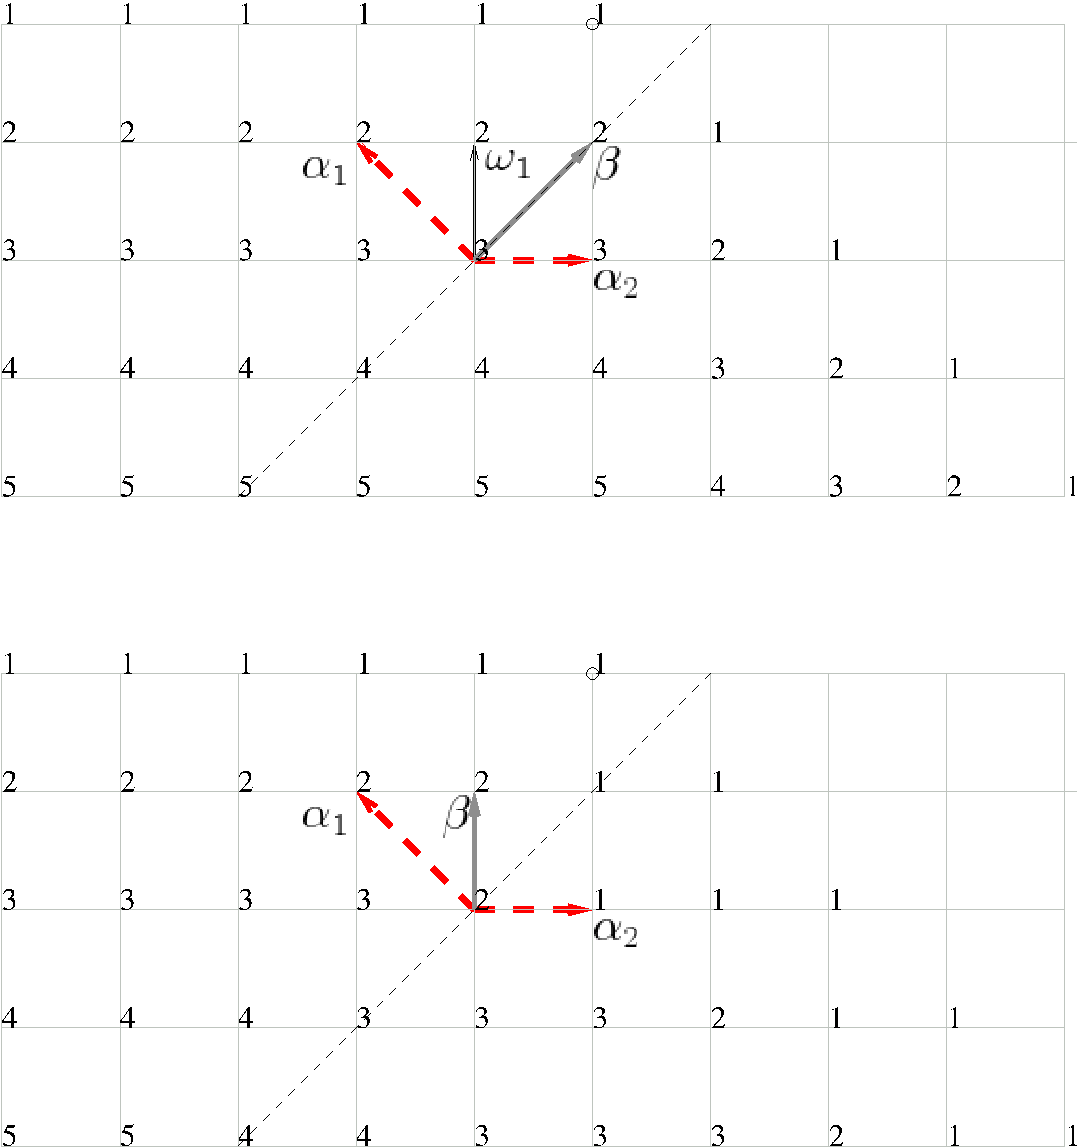
\includegraphics[width=120mm]{B2_Verma_Branch3}
  }
  \caption{Branching for the Verma modules}
  
  \label{fig:B2_Verma_Branch2}
\end{figure}
In present paper we interpret this branching coefficients as the dimensions of the weight subspaces of the modules of contracted algebras.



\section{Regular subalgebras and generalized Verma modules}
\label{sec:regul-subalg-gener}

Let us state the following lemma.
\begin{lemma}
\label{lemma-1}
The quotient of the singular weights element $\Psi^{(\mu)}$ by the denominator $R_{\af_{\bot}}$ is given by the formal element corresponding to the modified set of the singular weights of $L_{\af\oplus\mathfrak{h}_d}^{(\pi_{\af\oplus\mathfrak{h}_d}\mu)}$ with the multiplicities given by the dimensions of $\af_{\bot}$-modules.
\begin{equation}
  \label{eq:4}
  \frac{\Psi^{(\mu)}_{\mathfrak{g}}}{\prod_{\alpha\in \Delta^{+}_{\afb}}\left(1-e^{-\alpha}\right)^{\mathrm{mult}(\alpha)}}=
    \sum_{u\in W/W_{\afb}}\epsilon(u)e^{\pi_{\tilde\af}\left[(u(\mu+\rho)-\rho)\right]+\mathcal{D}}\cdot \mathrm{ch}_{\af_{\bot}}
      L^{\piab(u(\mu+\rho)-\rho)-\mathcal{D}}
\end{equation}
\end{lemma}  
\begin{proof}
  Consider $\Psi^{(\mu)}_{\mathfrak{g}}$. It is given by the sum over the Weyl group.
  \begin{equation}
    \label{eq:6}
    \Psi^{(\mu)}_{\mathfrak{g}}=\sum_{w\in W}\epsilon(w)e^{w(\mu+\rho)-\rho}
  \end{equation}
  We can divide the summation to the sum over $W_{\afb}$ and sum over all the classes of $W/W_{\afb}$: $w=vu,\; v\in W_{\afb},\; u \in W/W_{\afb}$. We have the following obvious property of the projections:
  \begin{equation}
    \label{eq:5}
    u(\mu+\rho)=\pia(u(\mu+\rho))+\piab(u(\mu+\rho))+\pi_{h_{\perp}^*}(u(\mu+\rho))
  \end{equation}
 Since $\mathfrak{h}_{\af}^*,\mathfrak{h}_{\perp}^*$ are invariant under the action of $v\in W_{\afb}$, we have
  \begin{equation}
    \label{eq:8}
    vu(\mu+\rho)-\rho=v\cdot(\piab(u(\mu+\rho))-\rho_{\afb}+\rho_{\afb})-\rho_{\afb}+\pia(u(\mu+\rho))-\rho+\rho_{\afb}+\pi_{\hf_{\perp}^*}(u(\mu+\rho))
  \end{equation}
  Only the first term depends on $v$. So
  \begin{equation}
    \label{eq:9}
    \frac{\Psi^{(\mu)}_{\mathfrak{g}}}{\mathrm{R}_{\afb}}=
    \frac{\sum_{u\in W/W_{\afb}}\epsilon(u)e^{\pia(u(\mu+\rho))-\rho+\rho_{\afb}+\pi_{\mathfrak{h}_{\perp}}(u(\mu+\rho))}\cdot
      \sum_{v\in W_{\afb}}\epsilon(v)e^{v(\piab u(\mu+\rho)-\rho_{\afb}+\rho_{\afb})-\rho_{\afb}}}{\mathrm{R}_{\afb}}
  \end{equation}
  We can rewrite the r.h.s. as
  \begin{equation}
    \label{eq:10}
    \sum_{u\in W/W_{\afb}}\epsilon(u)e^{\pi_{(\af\oplus\mathfrak{h}_d)}\left[u(\mu+\rho)-\rho\right]+\pi_{(\af\oplus \mathfrak{h}_d)}\cdot \rho-\rho+\rho_{\afb}}\cdot
    \mathrm{ch}_{\afb}L^{\pi_{\afb}u(\mu+\rho)-\rho_{\afb}}.
  \end{equation}
  Since $\pi_{\afb}(u(\mu+\rho)-\rho)-(\rho_{\afb}-\pi_{\afb}\rho)=\pi_{\afb}(u(\mu+\rho)-\rho)-\mathcal{D}$ and $\pi_{\tilde\af}\rho-\rho=-\pi_{\afb}\rho$ we get the statement of the Lemma.

\end{proof}

\begin{corollary}
  \label{sec:corollary-1}
  If we apply the projection $\pi_{\af}$ to the subalgebra $\af$ to the equation (\ref{eq:4}) we obtain the ``Lemma 1'' from the paper \cite{2010arXiv1007.0318L} in the case of regular subalgebras $\af, \afb$. However this Lemma \ref{lemma-2} is more general then Lemma \ref{lemma-1}, since it holds for the special subalgebra $\af$.
\begin{lemma}
\label{lemma-2}
Let $\af$ and $\af_{\perp }$ be the orthogonal pair of regular
subalgebras in $\frak{g}$, with $\widetilde{\af_{\perp }}=\af%
_{\perp }\oplus \frak{h}_{\perp }$ and $\widetilde{\af}=\af\oplus
\frak{h}_{\perp }$ ,

$L_{\frak{g}}^{\mu }$ be the highest weight module with the singular element
$\Psi _{\frak{g}}^{\mu }$ ,

$R_{\af_{\perp }}$ be the Weyl denominator for $\af_{\perp }$.

Then the element $\pi _{\af}\left( \frac{\Psi _{\frak{g}}^{\mu }}{R_{%
\af_{\perp }}}\right) $ can be decomposed into the sum over $u\in U$ (see (\ref{U-def})) of
the singular elements $e^{\mu _{\af}\left( u\right) }$ with the
coefficients $\epsilon (u)\mathrm{\dim }\left( L_{\widetilde{\af_{\perp
}}}^{\mu _{\widetilde{\af_{\perp }}}\left( u\right) }\right) $:
\begin{equation}
\quad \pi _{\af}\left( \frac{\Psi _{\frak{g}}^{\mu }}{R_{\af%
_{\perp }}}\right) =\sum_{u\in U}\;\epsilon (u)e^{\mu _{\af}\left(
u\right) }\mathrm{\dim }\left( L_{\widetilde{\af_{\perp }}}^{\mu _{%
\widetilde{\af_{\perp }}}\left( u\right) }\right) .
\label{eq:11}
\end{equation}
\end{lemma}
This lemma can be used to state the recurrent relation for the branching coefficients for the reduction of $\gf$-module to $\af$-modules. (See \cite{2010arXiv1007.0318L} for the details). It will be also useful for the discussion of special subalgebras. 
\end{corollary}
\begin{corollary}
  \label{corollary-2}
 If $\af, \afb$ are regular subalgebras the simple root system $\alpha_1,\dots, \alpha_r$ of $\gf$ sometimes can be chosen in such a way that simple roots $\beta_1,\dots,\beta_{r_{\afb}}$ of $\afb$ are contained in it. Denote the set of roots $\beta_i$ by $I$. This notation is in the agreement with the book \cite{humphreys2008representations}.
  \begin{equation*}
    I=\{\beta_1,\dots,\beta_{r_{\afb}}\}\subset \{\alpha_1,\dots,\alpha_r\}
  \end{equation*}
  Then the subset $I$ determines not only the subalgebra $\afb$, but also the minimal parabolic subalgebra $\mathfrak{p}_I$, such that $\afb\subset \mathfrak{p}$. Then we can consider the modules of the subcategory $\mathcal{O}^{\mathfrak{p}}$, for example the generalized Verma modules $M_{\mathfrak{p}}^{(\mu)}$. This modules are constructed from the irreducible highest-weight modules $L_{\pf}^{(\mu)}$ as follows
  \begin{equation}
    \label{eq:1}
    M_{\pf}^{(\mu)}=U(\gf)\otimes_{U(\pf)} L^{(\mu)}_{\pf}
  \end{equation}
  Denote by $\tilde R$ the denominator constructed of the positive roots of $\gf$ which are not the roots of $\afb$.
  \begin{equation}
    \label{eq:2}
    \tilde R = \prod_{\alpha\in \Delta^+\setminus \Delta^{+}_{\afb}} \left(1-e^{-\alpha}\right)^{\mathrm{mult}_{\gf} \alpha}
  \end{equation}
If we expand $\frac{1}{\tilde R}$ the coefficients near the terms $e^{\xi}$ are given by the Kostant partition function $p^I$ constructed from the roots of $\gf$ which are not in $I$. 
The character of the generalized Verma module then can be formally written as
\begin{equation}
  \label{eq:3}
  \mathrm{ch} M^{(\mu)}_{\pf}=\frac{1}{\tilde R} \mathrm{ch}L^{(\mu)}_{\pf}
\end{equation}
The character of the irreducible finite-dimensional $\pf$-module $L^{(\mu)}_{\pf}$ differs from the character of the irreducible finite-dimensional $\afb$-module by the factor $e^{\pi_{\tilde\af}(\mu)}$, since $\pf$ contains the full Cartan subalgebra $\hf\subset\gf$.
Now if we multiply the statement (\ref{eq:4}) of the lemma \ref{lemma-1} by $\frac{1}{\tilde R}$ we get the character of irreducible highest-weight module $L^{(\mu)}$ on the left and the sum of the characters of generalized Verma modules on the right-hand side of the equation:
\begin{multline}
  \label{eq:7}
  \mathrm{ch}L^{(\mu)}_{\gf}=
  \sum_{u\in W/W_{\afb}}\epsilon(u)e^{\pi_{\af\oplus\mathfrak{h}_d}\left[(u(\mu+\rho)-\rho)\right]+\mathcal{D}}\cdot \frac{1}{\tilde R}\mathrm{ch} L_{\afb}^{\piab(u(\mu+\rho)-\rho)-\mathcal{D}}=\\
  \sum_{u \in W/W_{\afb}} \epsilon(u) \mathrm{ch} M^{(u(\mu+\rho)-\rho)}_{\pf}
\end{multline}
So we have recovered the Bernstein-Gelfand-Gelfand resolution \cite{bernstein1976category,bernstein1975differential,bernstein1971structure} for the parabolic category ${\cal O}^{\pf}$.
\end{corollary}

Note, that not all the examples of branching lead to the generalized Verma modules. For example,
consider the embedding $\af_{1}=B_{4}\subset \gf=B_{6}$. As we mentioned in \cite{2010arXiv1007.0318L} the
orthogonal subalgebra $\afb=B_{2}$. Then consider the regular subalgebra $\af=A_{1}\subset
\af_{1}\subset \gf$ with the root system spanned over the first long root of $\af_{1}$. Its
orthogonal subalgebra in $\gf$ contains the root systems of two algebras $B_{2}$. But those two root
systems cannot be built on the simple roots of $\gf$.
\section{Generalizations}
\label{sec:generalizations}

\begin{enumerate}
\item If $\af$ is a special subalgebra of $\gf$, the equation (\ref{eq:4}) and the Lemma \ref{lemma-1} no longer holds since the module of the algebra can not be presented as the composition of the modules of the subalgebra. Only the projection of this module can be decomposed. So we have to rely on the Lemma \ref{lemma-2}, which holds in this case too \cite{2010arXiv1007.0318L}.

Again as in the Corollary \ref{corollary-2} we can multiply the equation (\ref{eq:11}) by the (projection of) the denominator $\frac{1}{\tilde R}$. This projection if well-defined due to the construction of $\afb$.
\begin{equation}
  \label{eq:12}
  \pi_{\af}\left(\mathrm{ch} L^{(\mu)}_{\gf}\right)= \sum_{u\in U}\epsilon(u) \pi_{\af}\left(\frac{1}{\tilde R}\right) e^{\mu_{\af}(u)}\mathrm{dim} \left( L_{\widetilde{\af_{\perp }}}^{\mu _{%
\widetilde{\af_{\perp }}}\left( u\right) }\right) .
\end{equation}
Since the subalgebra $\afb$ is regular by construction,  at the right-hand side of the equation we see the generalized Verma module character projected on the root space of $\af$. So we have recovered the equation (\ref{eq:7}) in the projected form.
\begin{equation}
  \label{eq:13}
   \pi_{\af}\left(\mathrm{ch} L^{(\mu)}_{\gf}\right)= \pi_{\af}\left(  \sum_{u \in W/W_{\afb}} \epsilon(u) \mathrm{ch} M^{(u(\mu+\rho)-\rho)}_{\pf}\right)
\end{equation}
We have also lost any trace of subalgebra $\af$. But we can rewrite the left-hand side as the combination of the irreducible highest weight modules of subalgebra $\af$
\begin{equation}
  \label{eq:14}
  \sum_{\nu\in P^{+}_{\af}} b^{(\mu)}_{\nu} \mathrm{ch} L^{(\nu)}_{\af}= \sum_{u \in W/W_{\afb}} \epsilon(u) \pi_{\af}\left(   \mathrm{ch} M^{(u(\mu+\rho)-\rho)}_{\pf}\right)
\end{equation}
Using the Bernstein-Gelfand-Gelfand resolution for the subalgebra $\af$ we get the expression which links the projected characters of generalized Verma modules with the characters of Verma modules of special subalgebra:
\begin{equation}
  \label{eq:15}
  \sum_{\nu\in P^+_{\af}}b^{(\mu)}_{\nu}\sum_{ w\in W_{\af}} \epsilon(w) \mathrm{ch} M_{\af}^{w(\mu+\rho_{\af})-\rho_{\af}} =  \sum_{u \in W/W_{\afb}} \epsilon(u) \pi_{\af}\left(   \mathrm{ch} M^{(u(\mu+\rho)-\rho)}_{\pf}\right)
\end{equation}

\end{enumerate}

% \section{Applications}
% \label{sec:applications}
% 
% \section{Conclusion}
% \label{sec:conclusion}
% 
% 
% \section{Acknowledgements}
% 
% The work was supported in part by RFFI grant N 09-01-00504 and the National
% Project RNP.2.1.1./1575.
% 
\section*{References}
\bibliography{article}{}
\bibliographystyle{utphys}
\end{document}
